\section{Lecture des acquisitions et premiers résultats}\label{sec:lecture-des-acquisitions-et-premiers-resultats}
   Maintenant que nous savons utiliser les récepteurs GNSS et enregistrer les mesures ainsi prises dans un fichier au format NMEA, vient désormais le moment de lire ces données avec Python afin de pouvoir les exploiter.

   \subsection{Implémentation}\label{subsec:implementation}
      Afin de rendre l'exploitation des données plus simple, plusieurs choix techniques ont été pris.
      Tout d'abord, la programmation en Python qui nous a paru adaptée à la forme du problème, le langage permettant facilement de traiter des données numériques contenues dans un fichier texte.

      Deuxièmement, il a été décidé de concevoir un programme orienté-objet, et donc d'implémenter une classe \texttt{Data} dans laquelle seront stockées les données contenues dans un fichier NMEA, ce qui permet alors, à partir d'une unique lecture des données du fichier d'acquisition, d'opérer différentes exploitations.
      Ainsi, il est possible à partir d'un simple fichier contenant des données NMEA d'instancier un objet \texttt{Data} qui en extraira l'ensemble des données à son initialisation.
      Il est alors possible d'opérer diverses opérations telles que le tracé d'un chemin GPS ou encore une étude métrologique comparative entre deux objets \texttt{Data} distincts, le tout en lisant une seule fois les données depuis le fichier texte.

      Nous allons donc, par la suite, détailler quelques opérations effectuées sur les données acquises.


   \subsection{Nettoyage des données}\label{subsec:nettoyage-des-donnees}
      Une première opération pouvant être effectuée sur les données est un \og nettoyage \fg{} de ces dernières, permettant de transformer les données brutes en des données pouvant être extraites vers une liste Python, permettant également le transtypage de données numériques en entiers ou flottants.

   \subsection{Visualisation des données}\label{subsec:visualisation-des-donnees}
      Une première visualisation des données possible à partir des données NMEA est, à partir des trames GGA (position du récepteur), l'évolution de la position du récepteur GNSS en deux dimensions (latitude et longitude).
      Ainsi, très simplement, les coordonnées extraites des trames GGA sont converties du format sexagésimal au format décimal afin d'être placées dans un repère 2D par le module \texttt{matplotlib} de Python, mais il est aussi possible de prendre en compte l'altitude, renseignée dans les trames GGA, pour obtenir un tracé en 3 dimensions.

      \begin{figure}[h]
          \centering
          \begin{subfigure}[h]{.45\textwidth}
             \centering
             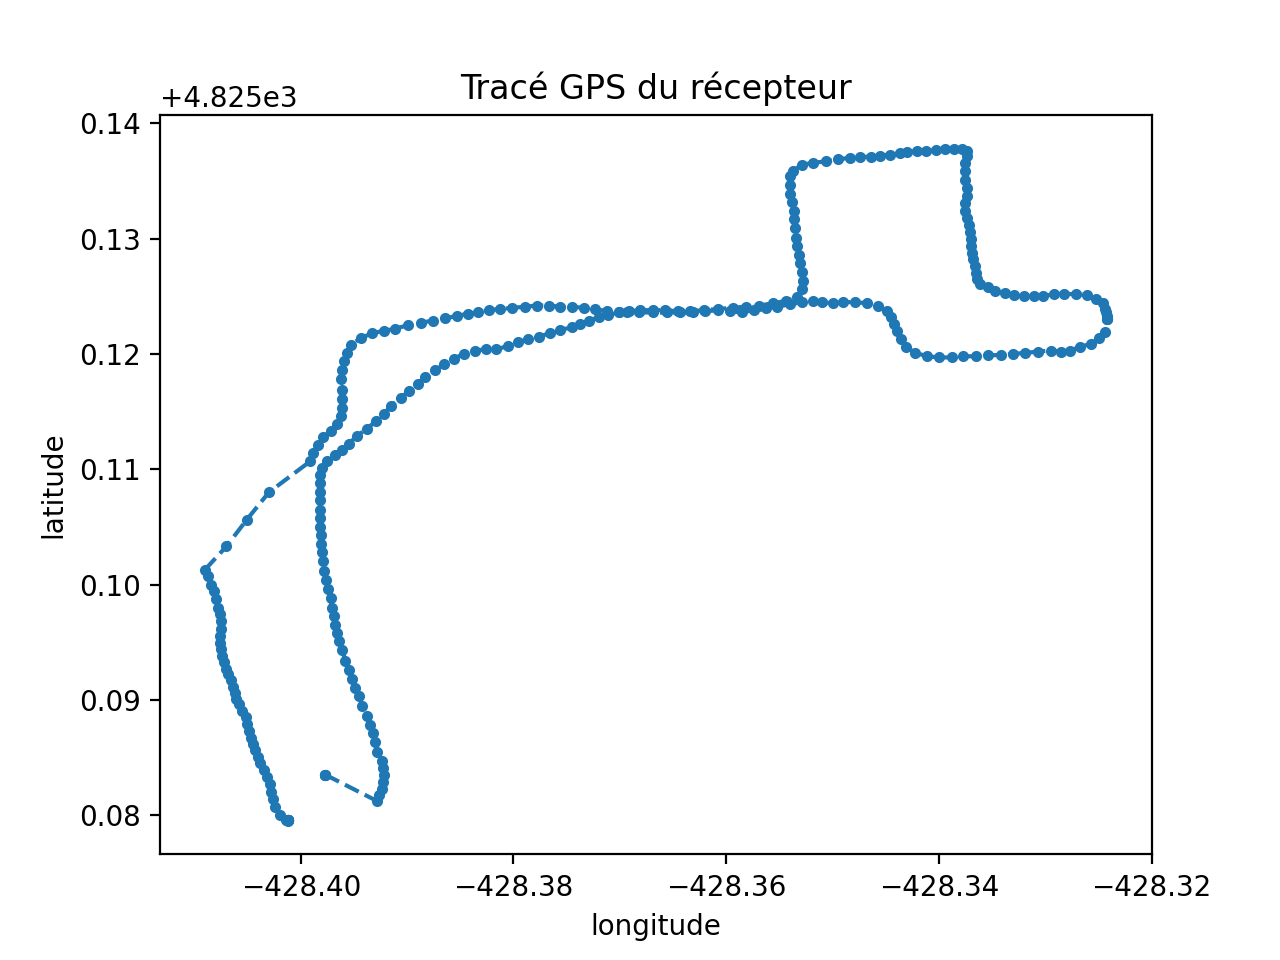
\includegraphics[width=\textwidth]{imgs/coords_2d}
          \end{subfigure}
          \hfill
          \begin{subfigure}[h]{.45\textwidth}
             \centering
             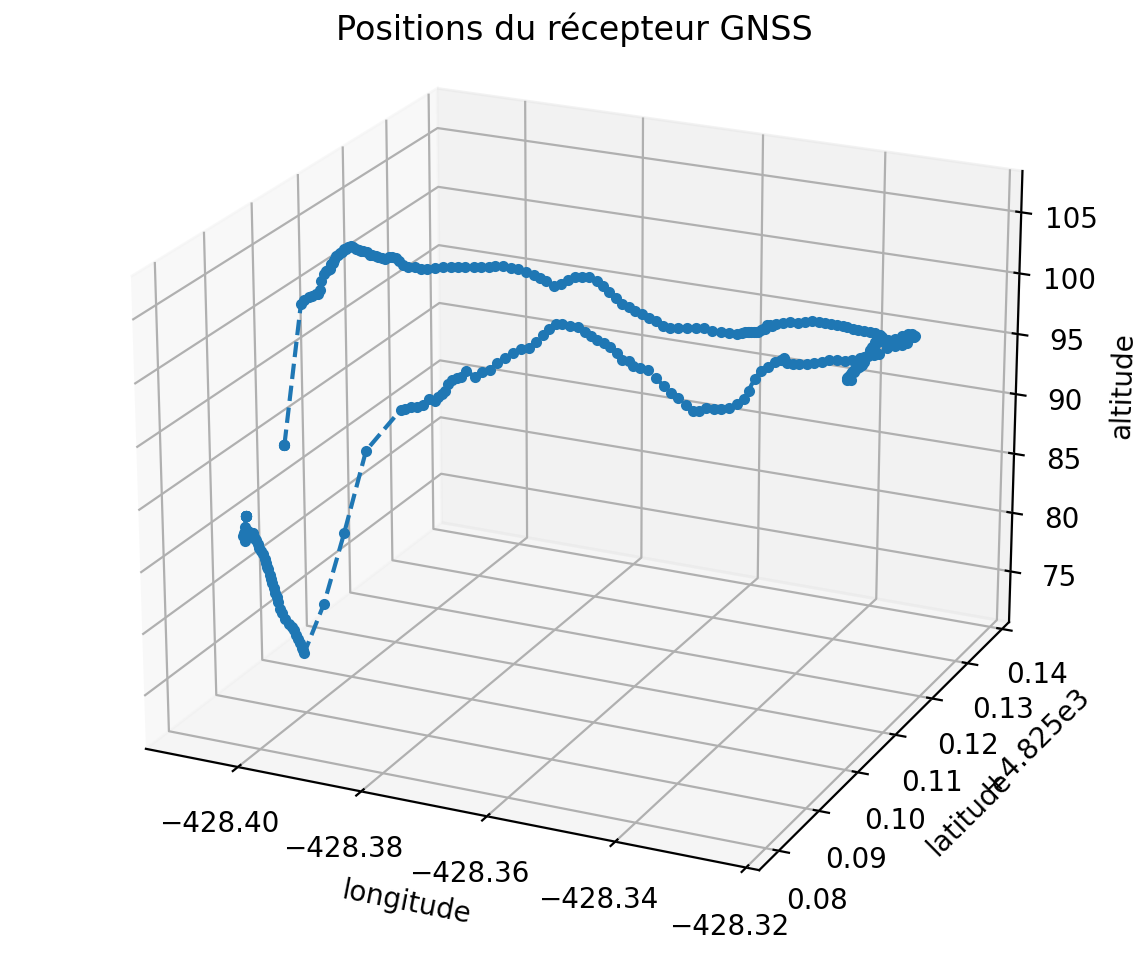
\includegraphics[width=\textwidth]{imgs/coords_3d}
          \end{subfigure}
          \caption{Position du récepteur en 2D et 3D}
          \label{fig:plot-coords}
      \end{figure}

      Mais il est également possible, grâce au module \texttt{folium}, d'obtenir la même représentation, mais sur un fond de carte\footnote{le fond de carte est celui d'\texttt{openstreetmap}} dans un fichier HTML (il est donc possible de naviguer sur la carte, sur laquelle est affiché le tracé des coordonnées successives du récepteur).

      \begin{figure}[h]
          \centering
          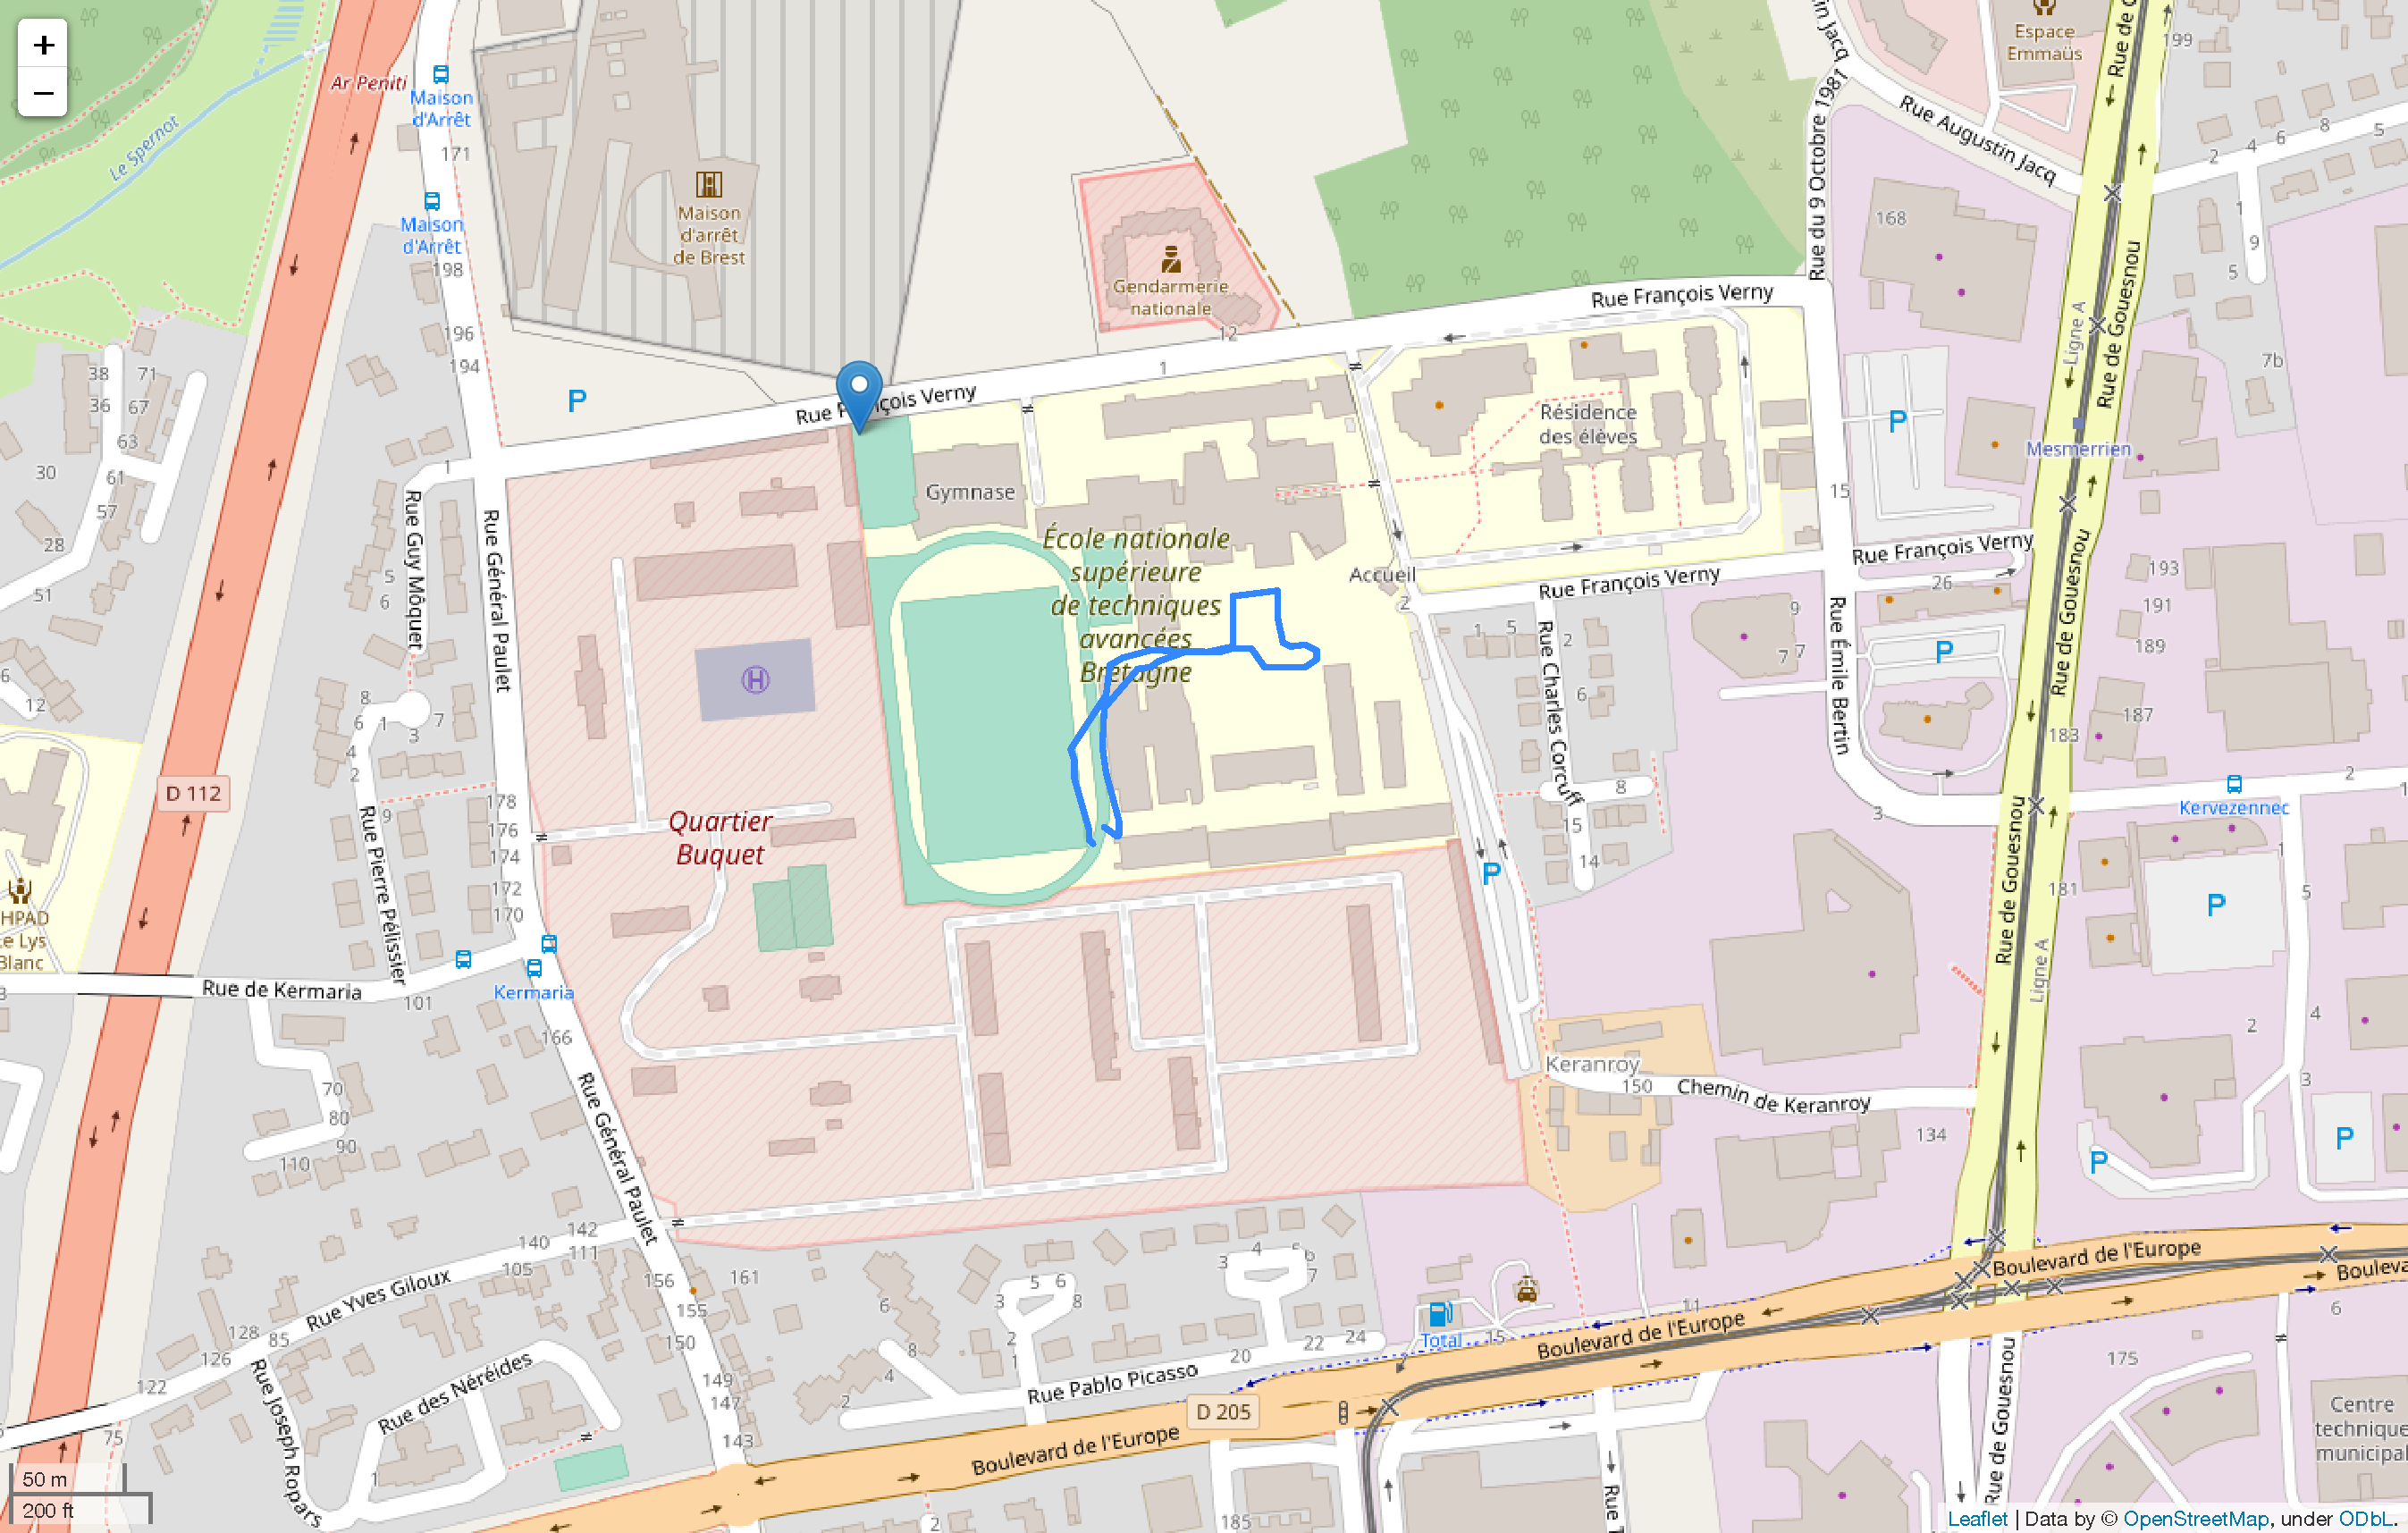
\includegraphics[width=.9\textwidth]{imgs/gps_map}
          \caption{Trace GPS sur un fond de carte HTML}
          \label{fig:coords-on-map}
      \end{figure}

